\chapter{Preliminaries}
\label{ch:preliminaries}

%-------------------------------------------------------------------------
\section{Data Synthesis}
\label{ch:preliminaries-dataSynthesis}

\subsection{Synthetic Data}
\label{ch:preliminaries-dataSynthesis-syntheticData}
Synthetic data can be defined as "(...) artificially generated data, that are modelled on real data, with the same structure and properties as the original data (...)" \cite[p. 2]{kaloskampis2020SyntheticDataCivil} 
but without containing any actual specific information or entries of the actual real data. 
While first synthetic data approaches \cite{gelman1992InferenceIterativeSimulation} focused on imputation techniques to generate synthetic data, the advent of deep learning has led to the topic gaining importance \cite{kowalczyk2022TaxonomyUseSynthetic, kaloskampis2020SyntheticDataCivil}
The importance of data is growing rapidly [TODO: QUELLE FINDEN] but accessing and collecting real data is usually expensive [TODO: QUELLE FINDEN] or simply not possible due to the sensitivity of the data (\eg medical records) \cite{esteban2017RealvaluedMedicalTimea} or due to regulatory restrictions, such as the \gls{gdpr} \cite{european_commission_regulation_2016}.
Synthetic data on the other hand is, compared to the collection of real data, cheap to generate \cite{leminh2021AirGenGANbasedSynthetica} and fulfils regulatory and privacy constraints \cite{zhao2022CTABGANEnhancingTabular}.

Hence, synthetic data could be used as an alternative to real data in various use-cases,
including but not limited to machine learning, software development or data sharing scenarios.
Access to data is still one of the biggest bottlenecks when developing machine learning or deep learning \glspl{model} \cite{fan2020RelationalDataSynthesisa}.
Synthetic data could be used to increase the data quality, by rebalancing skewed dataset \cite{zhao2022CTABGANEnhancingTabular} 
or increasing the dataset size as additional training data or in combination with the real data \cite{leminh2021AirGenGANbasedSynthetica, kim2021OCTGANNeuralODEbased}.
Synthetic data can also be used in situations where working with the real data is not possible, due to privacy or availability reasons [TODO: bessere quelle raussuchen]\cite{zhao2022CTABGANEnhancingTabular}.
In software development, high quality test data is crucial for development but challenging and time consuming to generate \cite{whiting2008CreatingRealisticScenariobased}.
Developers time to create such datasets is usually scarce and it might be the case that developers do not even have the permission to see the data, due to its sensitivity \cite{whiting2008CreatingRealisticScenariobased}.
A synthetic data generation \gls{model} would possibly allow developers to generate test data with predefined characteristics and without it being restricted in any form.


\subsection{Tabular Data}
\label{ch:preliminaries-dataSynthesis-tabularData}

Tabular data is the most one of the most common forms of structured data \cite{hernandez2022SyntheticDataGeneration} used to store, classify and share information \cite{pilaluisa2022ContextualWordEmbeddings}.
A table is made up of individual cell entries stored in rows and columns where rows can be seen as individual data points and columns are the different features \cite{borisov2022DeepNeuralNetworks, yoon2020VIMEExtendingSuccess}
This format is the most common way to maintain massive databases \cite{esmaeilpour2022BidiscriminatorGANTabular, yoon2020VIMEExtendingSuccess}.
and is crucial for applications that store heterogeneous information such as demographics, medical or financial information \cite{borisov2022DeepNeuralNetworks, yoon2020VIMEExtendingSuccess}.
Tabular data consists of multiple attribute types, such as categorical or continuous data types\cite{borisov2022DeepNeuralNetworks}.
While continuous values are of quantitative nature and stored in a numerical format, categorical values are made up by one value out of a limited set of values \cite{lederrey2022DATGANIntegratingExperta, lane2003IntroductionStatistics}.
Categorical attribute types can be further subdivided into binary, only two possible values, nominal, at least three possible values that do not follow any order and lastly ordinal with at least three entries where the values follow have an underlying order \cite{lederrey2022DATGANIntegratingExperta}.
This work adapts the formal definition of a table from \cite{xu2019ModelingTabularData}:

\begin{displayquote}
A table $T$ contains $N_{con}$ continuous columns and $N_{cat}$ categorical columns. [TODO: Definition ohne Discrete values]
\end{displayquote}

It is also possible that tabular data can contain other special data types like dates or timestamps which often contain information about the specific time a datapoint was recorded \cite{hernandez2022SyntheticDataGeneration}.
This kind of tabular data can be considered as dynamic tabular data, where individual records, \ie rows, can be dependent on each other, also known as a multivariate time series \cite{padhi2021TabularTransformersModeling}.
In static tabular data on the other hand the individual rows are independent from each other \cite{padhi2021TabularTransformersModeling}.
Hence, the order of rows and columns does not carry any meaning \cite{somepalli2021SAINTImprovedNeural}.
While the order of rows and columns does not matter, the individual values in one cell may vary well depend on values of another cell \cite{lederrey2022DATGANIntegratingExperta}.
An example for such an interdependency could occur in a demographics table, where an individual's legal status may depend on their age, 
for instance, a person under 18 years old is considered a minor and has different legal rights and responsibilities compared to an adult.

The authors of \cite{borisov2022DeepNeuralNetworks} identify four possible challenges when working with tabular data in a learning context.
The first identified challenge is the low quality of the data. Typical quality issues include missing values, noise in the data, extreme data points, data inconsistencies, class imbalance or high dimensionalities after preprocessing \cite{borisov2022DeepNeuralNetworks}[CONFIRM 1].
Secondly the missing irregular spatial dependencies of tabular data. Other common data formats like images or audio are homogeneous, 
meaning that they consists of only 1 feature type \cite{borisov2022DeepNeuralNetworks}.
Since tabular data consists of multiple features, made up of a mixture of categorical and numerical values, it is a heterogeneous data format with data points as rows and features as columns \cite{borisov2022DeepNeuralNetworks}.
This makes is especially challenging for neural networks to work with since the correlations between the features is weaker because they often do not have any form of spatial or semantic relationship like image or text data has \cite{borisov2022DeepNeuralNetworks, yoon2020VIMEExtendingSuccess}.
The third challenge is about the dependency on preprocessing. \cite{borisov2022DeepNeuralNetworks} highlights the importance of a preprocessing and explicit feature construction step that is necessary when working with tabular data in a deep learning context.
This preprocessing step is crucial since it does not only strongly influences the performance of deep learning \glspl{model} \cite{gorishniy2022EmbeddingsNumericalFeatures} 
it also introducing new challenges. 
Depending on the preprocessing strategy (\autoref{sec:preprocessing}) it is possible to create a very sparse feature matrix, create a synthetic ordinal ordering of a nominal variable or lose some information during the conversion of the data \cite{borisov2022DeepNeuralNetworks}.
The last and fourth challenge concerns the importance of a single feature. In homogeneous data multiple features need to change in order to change the class of the data. 
For heterogeneous tabular data a small change in one feature variable can already alter the class of the row. 
\cite{borisov2022DeepNeuralNetworks} illustrates this with the example of an image, where multiple pixels (\ie features) need to change in a coordinated manner in order to change the content (\ie class) of the image.
For tabular data a single change in a cell can change the prediction of a predictive \gls{model} \cite{borisov2022DeepNeuralNetworks}. 
Consider a \gls{model} that has to predict whether an individuals income is higher or lower than US\$ 50.000 per year \cite{Dua:2019} based on demographic information of that individual.
Switching an individuals "education" value from "Preschool" to "Doctorate" would likely cause the prediction to change from "<=50K" to ">50K".



\subsubsection{Tabular Data Preprocessing}
\label{sec:preprocessing}

Different data types can and should be processed into a meaningful format to be useful for deep learning \glspl{model} in different ways \cite{fan2020RelationalDataSynthesisa, lederrey2022DATGANIntegratingExperta}.
It is usually the first step before working with the data on any task \cite{izonin2022TwoStepDataNormalization}.
Data preprocessing itself consists of multiple different tasks: Data cleaning, data normalization, data transformation, data integration, missing value imputation and noise identification \cite{garcia2016BigDataPreprocessing}
While each of the preprocessing tasks is in itself important, 
\cite{fitkov-norris2012EvaluatingImpactCategorical} and \cite{gorishniy2022EmbeddingsNumericalFeatures} showed that a proper transformation of categorical and numerical entries respectively can have a significant influence on a deep learning \glspl{model} performance.
\cite{xu2019ModelingTabularData} showed the importance of normalization for synthetic tabular data generation.
Since the focus of the work is on tabular data and its synthesis, the following section will highlight the most important tabular data transformation and normalization approaches.

\subsubsubsection{Data Transformation}
\label{sec:dataTransformation}

\cite{borisov2022DeepNeuralNetworks} introduces a taxonomy for data transformation methods and subdivides the existing approaches into "Single-Dimensional Encodings" and "Multi-Dimensional Encodings".
The goal is to transform the different values column can take and transform them into a different (numeric) representation, such that it can be processed by a deep learning \gls{model}.

\textbf{Single-Dimensional Encodings:}
Single-Dimensional encoding techniques encode each cell independently \cite{borisov2022DeepNeuralNetworks}.
The following approaches are common techniques to encode a categorical column entry, usually in a text format, into a numerical format.
In ordinal- (or label-) encoding a simple mapping from each category to a numeric value occurs. 
While this introduces a synthetic ordering of potentially unordered categories, one-hot encoding overcomes this issue by introducing a new vector with the length of all possible values a categorical column can take.
All values in this vector are assign to zero except one entry that represents the category that should be encoded, which is set to one.
However, this approach can lead to high dimensionality feature vectors if the cardinality of the unique categories in categorical columns is large.
Binary encoding tries to reduce the dimensionality by setting the vector length to a maximum of $log(c)$ for $c$ unique categorical values in a column.
Each possible value is mapped to a number like in ordinal-encoding starting at 0 but the number is represented as a binary vector.
The leave-one-out encoding technique is an approach to encode a categorical column based on the target column in a machine learning scenario. 
A categorical entry is replaced by the mean of the target variable of all rows where the same category is present, excluding the target value of the to be encoded value.
Lastly, a hash-based approach is worth mentioning, where a deterministic hash function transforms each category into a numerical form \cite{borisov2022DeepNeuralNetworks}.

Numerical data, such as integers or floating point numbers, can often be used directly in deep learning \glspl{model} without undergoing a special encoding process. 
This is because deep learning algorithms are designed to handle numerical data and can learn patterns and relationships within the data without the need for additional encoding.
However, \cite{gorishniy2022EmbeddingsNumericalFeatures} has shown that in some cases, encoding numerical data can improve the performance of deep learning \glspl{model}. 
Encoding numerical data can be achieved through various methods such as normalization (see \autoref{sec:dataNormalization}), discretization, or using embeddings.

%Die beiden abschnitte auslagern in eigenen abschnitt? (GGF nur embeddings auslagern?)
Discretization techniques transform numerical features to categorical features, hence, quantitative data into qualitative data \cite{garcia2016BigDataPreprocessing}. 
\cite{dougherty1995SupervisedUnsupervisedDiscretization} gives an overview on classical discretization techniques, such has equal interval width binning, where the continues values are divided and assign to certain amount of bins.
A modern approach by researchers from NVIDIA \cite{dong2022GeneratingSyntheticData} invented a tokenizer specifically for tabular data with float numbers. 
This tokenizer converts float numbers into a sequence of token IDs \cite{dong2022GeneratingSyntheticData}.

In Embedding techniques values that should be encoded (\eg words or tabular cell entries) are mapped to a vector representation. 
This vector of real numbers tries to capture "semantic regularities in vector spaces" \cite[p. 2]{pilaluisa2022ContextualWordEmbeddings}.
The goal of embeddings is to create a vector space, in which semantically similar values are also numerically similar \cite{pilaluisa2022ContextualWordEmbeddings}.
It can be differentiated between static embeddings and contextualized embeddings. 
While the former embedding technique always provides the same numerical representation for an input value, the latter embedding technique changes the vector representation of value based on its surrounding context \cite{pilaluisa2022ContextualWordEmbeddings}.
This is especially important in the natural language processing domain, where contextual embeddings has led to state-of-the-art improvements \cite{pilaluisa2022ContextualWordEmbeddings}.
Homonyms or polysemic words like "bat" or "second" are words that carry multiple different meanings and their semantic meaning therefore changes with the context they are used in. [TODO: QUELLE]
Hence, the contextualized embedding vector of the word "second" in the context of time (\eg "it took me 3 seconds") should be different to the one where "second" is used in the context of a competition (\eg "he achieved the second place").
Contextualized embeddings have to be learned during some form of (pre-) training \cite{devlin2019BERTPretrainingDeep, iida2021TABBIEPretrainedRepresentations, deng2021TURLTableUnderstanding}. 
Static embeddings, such as Word2Vec \cite{mikolov2013DistributedRepresentationsWords} are learned as well. 
It is also possible to use the embedding layers to get a vector representation without learning, which can be seen as a "feature tokenization" \cite{zheng2022DiffusionModelsMissing, gorishniy2021RevisitingDeepLearning}.
However, semantic similarity in a vector space cannot be achieved without any learning, so this embedding technique is more similar to a discretization/tokenization technique.

[TODO: Insert example for single-dim encoding in tabular data]

\textbf{Multi-Dimensional Encodings:}
Multi-Dimensional encoding techniques focuses on encoding an entire record (or table-row) into another representation \cite{borisov2022DeepNeuralNetworks}.
The VIME framework \cite{yoon2020VIMEExtendingSuccess} uses a multilayer perceptron as an encoder that encodes a tabular input row into a latent representation, 
similar to the encoder of famous (variational-) auto-encoders \cite{kingma2013AutoEncodingVariationalBayes} architectures.
This latent representation is, like in embeddings, a learned representation learned through self-supervised learning tasks, feature vector estimation and mask vector estimation \cite{yoon2020VIMEExtendingSuccess}.
\cite{borisov2022DeepNeuralNetworks} also lists other multi-dimensional encoding techniques, such as the works of \cite{zhu2021ConvertingTabularData} and \cite{sun2019supertml}.
Both architectures transform tabular data into an image like format in order to make use of \glspl{cnn}.


\subsubsubsection{Data Normalization and Standardization}
\label{sec:dataNormalization} 

Normalization and standardization techniques are applied to numerical columns and scales the values so that their distribution is adjusted \cite{garcia2016BigDataPreprocessing}.
This is especially important in tabular data, where numerical features are likely having a different scale, \eg a column "age" could have a range of 1 to 100 and a column income could have a range from 0 to 1 million [TODO: Quelle finden].
Normalization allows to scale each column a similar range (usually 0 to 1, or -1 to 1) while maintaining the overall distribution of each column \cite{izonin2022TwoStepDataNormalization}.
Standardization on the hand rescales the data so it follow a normal distribution with mean 0 and standard deviation 1 \cite{scikit-learnPreprocessingData}.
Standardization and Normalization of values is especially important if the data will be used in a machine learning context, where machine learning models might behave unexpectedly if 
the features do not look similar to a gaussian distribution with zero mean and unit variance or are ranged between 0 and 1 \cite{scikit-learn, scikit-learnPreprocessingData}.
Through this data rescaling, the sensitivity of \gls{model} to large values is reduced and the generalizability is increased \cite{izonin2022TwoStepDataNormalization}.
The most common standardization and normalization approaches are probably the StandardScaler and the MinMaxScaler, respectively.
The StandardScaler standardizes a feature value $x_i$ according to the mean and standard distribution of the feature column, so it follows a normal distribution \cite{garcia2016BigDataPreprocessing, izonin2022TwoStepDataNormalization}.
It can be defined as $x' = \frac{x_i-mean(x)}{std(x)}$, with $x'$ as the standardized $x_i$ value \cite{izonin2022TwoStepDataNormalization}.
The MinMaxScaler on the other hand makes use of the maximum and minimum of each feature column and scales the values accordingly.
It is defined as $x' = \frac{x_i - min(x)}{max(x) - min(x)}$ \cite{izonin2022TwoStepDataNormalization}.
While the StandardScaler is usually used for data that follows a gaussian normal distribution, MinMaxScaler is better suited for arbitrary distributions [TODO: QUELLE finden].
A more complex normalization technique addresses the problem, that numeric values in tabular data can follow distributions more complex than just a simple gaussian normal distribution \cite{zhao2022CTABGANEnhancingTabular, xu2019ModelingTabularData}.
\cite{xu2019ModelingTabularData} introduces mode-specific normalization which models complex distributions with multiple simple gaussian distributions.
\cite[p. 3-4]{xu2019ModelingTabularData} defines the mode-specific normalization technique in following way:

\begin{enumerate}
    \item For each continuos column $C_i$, estimate the number of modes $m_i$ by using a \gls{vgm} \cite{bishop2006PatternRecognitionMachine}. 
    For example, in \autoref{fig:mode-specific-normalization} the \gls{vgm} estimates $m_i=3$, $\eta_1$, $\eta_2$ and $\eta_3$. 
    The learned gaussian mixture is  
    $\mathbb{P}_{C_i}(c_{i,j})=\sum_{k=1}^{3}\mu_k\mathcal{N}(c_{i,j};\eta_k, \sigma_k)$
    with $\mu_k$ and $\sigma_k$ as weight and standard deviation of a mode respectively.
    \item For each $c_{i,j}$ the probability is calculated of $c_{i,j}$ coming from each mode. 
    In \autoref{fig:mode-specific-normalization}, $p_1$, $p_2$ and $p_3$ denote the probability densities, calculated as $p_k=\mu_k\mathcal{N}(c_{i,j};\eta_k;\sigma_k)$.
    \item Given $p_1$, $p_2$ and $p_3$ for $c_{i,j}$ sample one mode and use it to normalize the value. 
    In the example of \autoref{fig:mode-specific-normalization}, $p_3$ is most likely and is sampled.
    The mode selection for $c_{i,j}$ is represented as a one-hot vector $\beta_{i,j}=[0,0,1]$ indicating that the third mode has been sampled.
    The actual value $c_{i,j}$ is normalized as $\alpha_{i,j}=\frac{c_{i,j}-\eta_3}{4\sigma_3}$. 
\end{enumerate}

The normalized representation $r$ of $c_{i,j}$ will be the concatenation of $\alpha_{i,j}$ and $\beta_{i,j}$: 

$r=\alpha_{i,j}\oplus\beta_{i,j}$

% include image from paper
\begin{figure}[h]
    \centering
    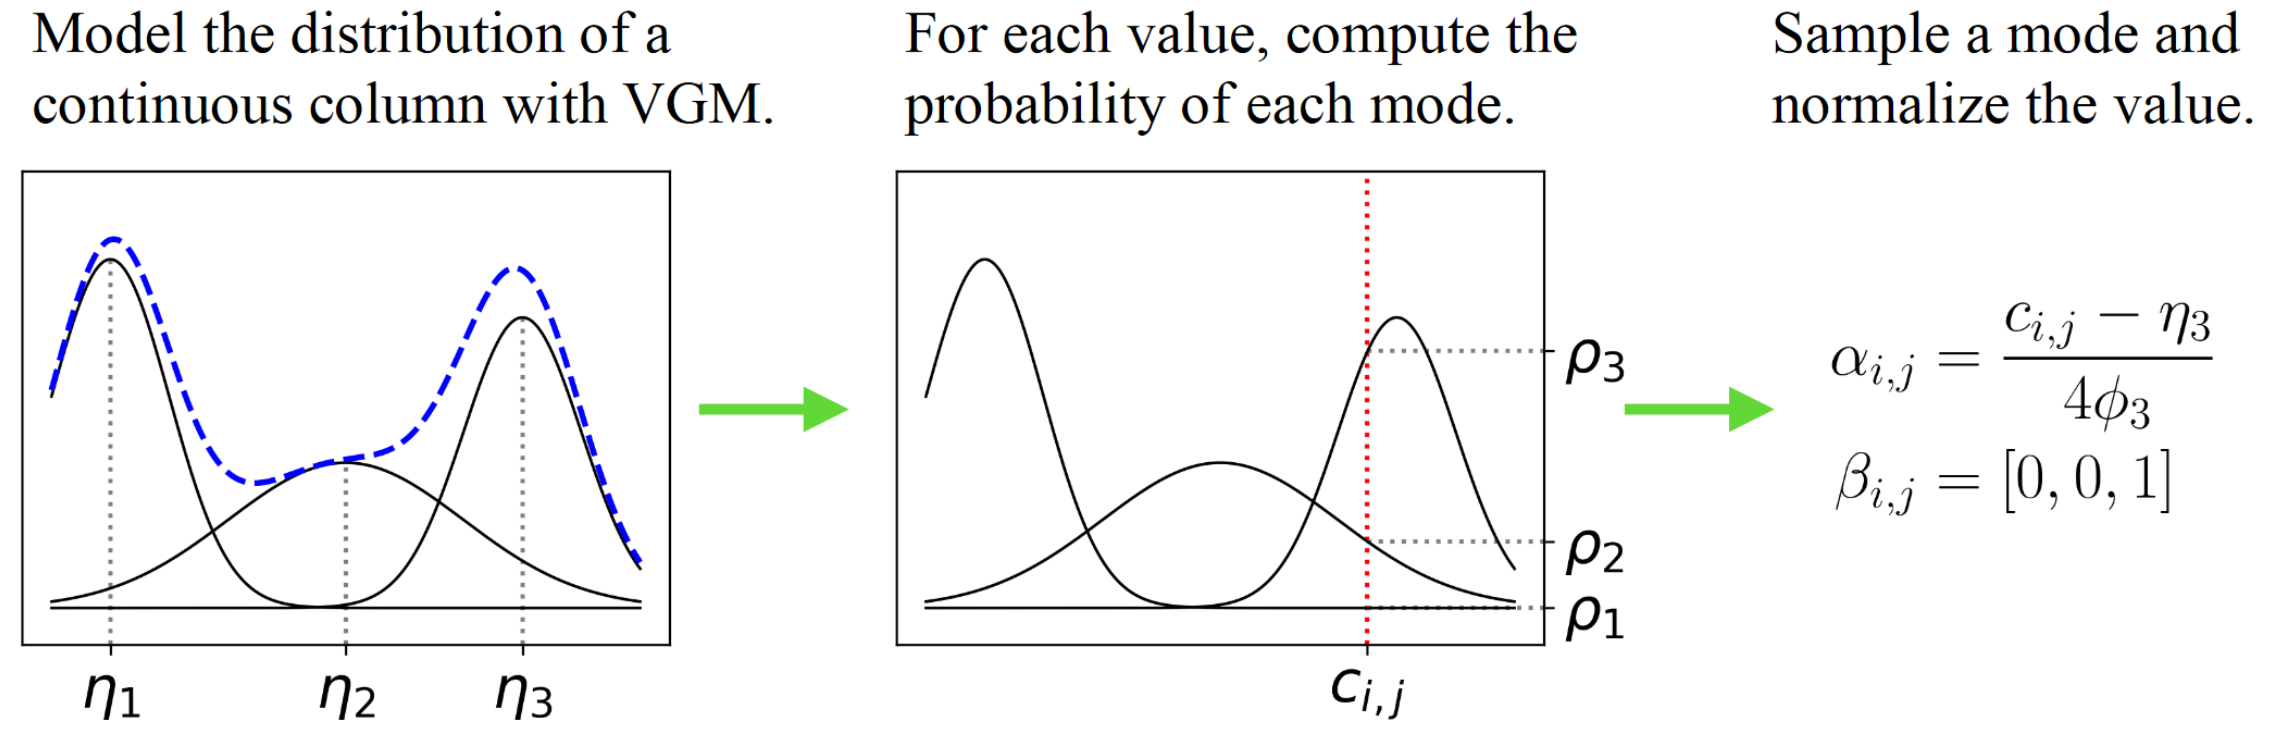
\includegraphics[width=0.5\textwidth]{images/mode-normalization.png}
    \caption{An example of mode-specific normalization [TODO: COPYRIGHT?] \cite[Figure 1, p. 4]{xu2019ModelingTabularData}}
    \label{fig:mode-specific-normalization}
  \end{figure}


Another approach to standardize the range of a column between 0 and 1 is a Quantile-Transformation, a non-linear transformation \cite{scikit-learnPreprocessingData, kotelnikov2022TabDDPMModellingTabular}.
The Quantile-transformation allows to map all values of a random variable into an desired output distribution, such as the uniform or normal distribution, 
using the quantile function on the inverse cumulative distribution of the random variable. This transformation preserves the rank order of the values but distorts correlations and distances within and across features \cite{scikit-learnPreprocessingData}.

\subsection{Synthetic Tabular Data Generation}

Generative models have recently received a lot of attention, thanks to their impressive results generating a variety of data formats, 
such as images \cite{ho2020DenoisingDiffusionProbabilistic, dhariwal2021DiffusionModelsBeat, rombach2022HighResolutionImageSynthesis}, videos \cite{ho2022VideoDiffusionModels, Gen1Runway}, text \cite{radfordImprovingLanguageUnderstanding, 2022ChatGPTOptimizingLanguage} or music \cite{agostinelli2023MusicLMGeneratingMusic, martirosRiffusion}.

While synthetic data generation can be applied to various types of data, generating synthetic tabular data is a challenging task due to the complexity of the underlying joint distributions between variables.
This work adapts the formal definition of the tabular data generation adapted from \cite[p. 2]{xu2019ModelingTabularData}:

\begin{displayquote}
    A data synthesizer $G$ is trained on a table $T$ and then used to generate a synthetic table $T_{syn}$. % Vllt die definition einer tabelle nach oben packen und von oben übernehmen?
    $T$ consists of $N_c$ continuos columns ${C_1, ..., C_{N_c}}$ and $N_d$ categorical columns (or a discrete representation of it) ${D_1, ..., D_{N_d}}$
    Each column is considered to be a random variable and follows an unknown joint distribution $\mathbb{P}(C_{1:N_c},D_{1:N_d})$.
    One row $r_j=\{c_{1,j}, ...,c_{N_c,j}, d_{1,j}, ...,d_{N_d,j}\}$, $j \in\{1, ..., n\}$, is one observation from the joint distribution.
    $T$ is partitioned into a training set $T_{train}$ and test set $T_{test}$. 
    The synthesizer $G$ is trained on $T_{train}$ and afterwards used to sample independently individual rows to create $T_{syn}$.
\end{displayquote}

During the generation of synthetic tabular data there are two competing objectives, high data utility and low disclosure risk.
Data utility is concerned with how well the synthetic data accurately reflects the real data in terms of its underlying patterns and relationships.
Low disclosure risk on the other hand is concerned with the preservation of privacy and confidentiality of the information in the real training dataset $T_{train}$ \cite{little2021GenerativeAdversarialNetworksa}. 

Tabular data synthesis approaches can be summarized into Process and data driven methods \cite{goncalves2020GenerationEvaluationSynthetic}.
Process driven models focus on simulating real world processes and gather data during that simulation to create the synthetic dataset \cite{kowalczyk2022TaxonomyUseSynthetic}.
On the other hand, data driven approaches aim to generate synthetic data based on already existing real-world dataset \cite{kowalczyk2022TaxonomyUseSynthetic}.
This can be achieved by augmenting the existing dataset, \ie applying transformations to the existing datapoints to generate new datapoints \cite{kowalczyk2022TaxonomyUseSynthetic}s.
Another technique to generate synthetic data is to simply sample from the individual feature distributions of a dataset to generate new synthetic data \cite{kowalczyk2022TaxonomyUseSynthetic}.
Lastly, machine learning and deep learning algorithms can be used to learn the underlying joint distributions of the real data to generate new synthetic data \cite{kowalczyk2022TaxonomyUseSynthetic}. 

%challanges
The synthesis of tabular data is, compared to other data types, especially challenging due to its heterogeneity, potential weak correlations among feature and dependency on preprocessing \cite{borisov2022DeepNeuralNetworks, yoon2020VIMEExtendingSuccess, gorishniy2022EmbeddingsNumericalFeatures}.
To create a realistic synthetic dataset interdependencies that may exists between variables must be captured and 
it is possible that the \gls{model} overfits on the training data and generalizes relationships between features that are only present in training but not test data \cite{lederrey2022DATGANIntegratingExperta}
In addition to that, tabular data columns can follow complex distributions, that make the synthesization challenging.
\cite{zhao2022CTABGANEnhancingTabular} identifies the following four properties of tabular data:

\begin{enumerate}
    \item Single Gaussian variables: Data where its distribution follows a gaussian distribution \cite{zhao2022CTABGANEnhancingTabular}.
    \item Mixed data type variables: A single column can contain a mix of continuos and categorical values. 
    For instance, a "loan" column could hold information about the size of an individuals loan.
    The values in this column are mostly positive float values but can also take the value "-1" which indicates, that this person did not get approach for a loan.
    Such a special categorical value in an otherwise numerical column need to be considered when working with this column \cite{zhao2022CTABGANEnhancingTabular}.
    \item Long tail distributions: In real world data (especially sales data), it can occur that most occur "near the initial value of a distribution and rare cases towards the end" \cite[p. 3]{zhao2022CTABGANEnhancingTabular}.
    This results in a tail-like distribution.
    \item Skewed multi-mode continuous variables: Complex numerical distributions do not necessarily follow a single gaussian distributions.
    It is possible for their distribution to consist of multiple unknown distributions that are potential skewed as well. 
    Their conjunction as a whole makes up the complex distribution \cite{zhao2022CTABGANEnhancingTabular}.
\end{enumerate}

A successful tabular data generator should be able to recreate such properties of real data in their synthetic data counterpart.



%-------------------------------------------------------------------------
\section{Deep Learning Architectures}
\label{ch:preliminaries-deepLearningArchitectures}

Deep learning has rapidly become a dominant force in artificial intelligence, revolutionizing various fields including computer vision, natural language processing, and data generation. 
Complex architectures made up of many layers of artificial neural networks are used to build deep learning models.
These architectures have enabled the creation of highly accurate and efficient models that are capable of processing vast amounts of data. 
In recent years, the development of new deep learning architectures has been a key area of research, leading to the creation of powerful models.
This section will start with a high-level introduction into the most important architectural building blocks of a neural network.
Afterwards the most important deep learning \gls{model} architectures for generating data are presented.

\subsection{Neural Networks}
\label{ch:preliminaries-deepLearningArchitectures-neuralNetworks}

The most basic neural network is called a perceptron \autoref{fig:perceptron} \cite{rosenblatt1958PerceptronProbabilisticModel}.
It consists of a single input layer that is connected to an output node.
Each input node is connected with the output node via weight edges.
For all inputs, the input value is multiplied with each respective weight.
The sum of all input-weight multiplication serves as the input to an activation function, which is different depending of the task at hand.
The output is the prediction of the perceptron which is compared to the actual result, the label, and an error is calculated.
This error is used later on to update the weights of the individual nodes via backpropagation \cite{aggarwal2018NeuralNetworksDeep}.
The output of one node can also serve as the input to another node, so multiple layers of nodes are created.
This is refereed to as a \gls{mlp} or feed-forward neural network \autoref{fig:mlp}, 
because the information flows forward from input through the multiple layers in the middle (also called hidden layers) to the output \cite{aggarwal2018NeuralNetworksDeep, Goodfellow-et-al-2016}.
An \gls{mlp} tries to approximate some function $f^*$ by defining a mapping $y=f(x;\theta)$ by learning the values of the parameters $\theta$ (\ie the weights) that best approximate $f^*$ \cite{Goodfellow-et-al-2016}.
A simple \gls{mlp} is already able to learn any "reasonable" function, which is why they are also considered to be universal function approximators \cite{aggarwal2018NeuralNetworksDeep, hornik1989MultilayerFeedforwardNetworks}.


\begin{figure}
    \begin{subfigure}{0.45\textwidth}
      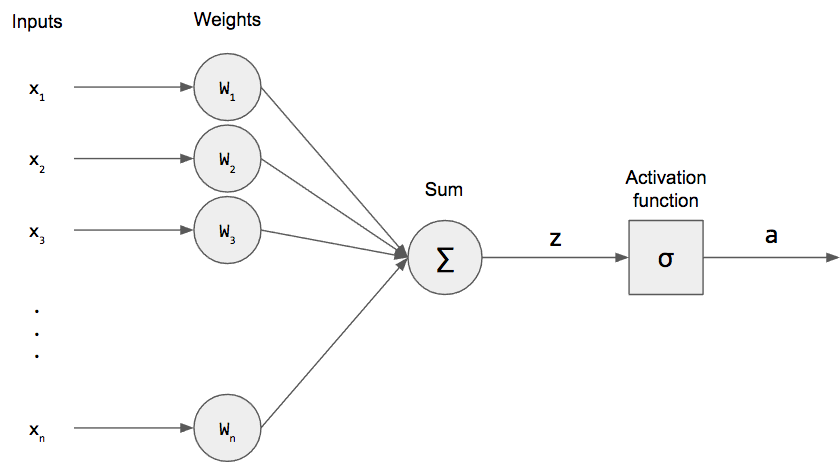
\includegraphics[width=\linewidth]{images/perceptron.png}
      \caption{Perceptron} \label{fig:perceptron}
    \end{subfigure}%
    \hspace*{\fill}   % maximize separation between the subfigures
    \begin{subfigure}{0.45\textwidth}
      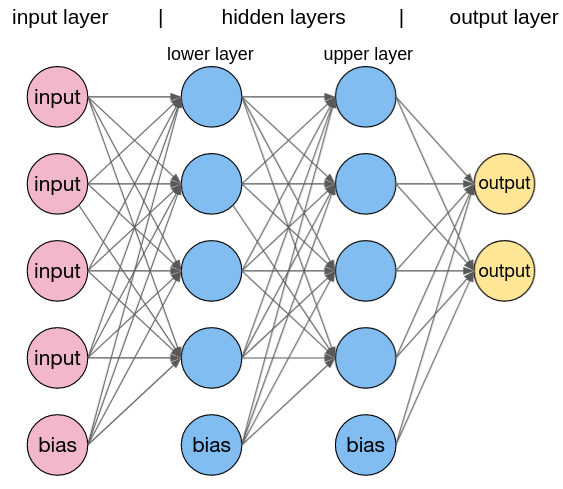
\includegraphics[width=\linewidth]{images/mlp.png}
      \caption{multilayer perceptron} \label{fig:mlp}
    \end{subfigure}%
    \hspace*{\fill}   % maximizeseparation between the subfigures
  \caption{Overview Neural Networks} \label{fig:NN_Overview}
\end{figure}





Convolutional networks, or \glspl{cnn} \cite{lecun1998GradientbasedLearningApplied}, are a specialized type of neural network.
As their name indicate, they perform convolutions on the data \autoref{fig:cnns}.
A convolution can be defined as "a dot-product operation between a grid-structured set of weights and similar grid-structured inputs drawn from
different spatial localities in the input volume" \cite[p. 316]{aggarwal2018NeuralNetworksDeep}.
They perform exceptionally well on data with a grid-like topology, with strong spatial dependencies, such as image or time-series data \cite{aggarwal2018NeuralNetworksDeep, Goodfellow-et-al-2016}.
In a typical convolutional network, a layer starts by performing multiple convolution operations in parallel on the data.
The linear activations that are produced by the convolutions are send through a nonlinear activation function (usually a \gls{relu}).
Lastly, a pooling function is applied to the output of the activation function.
A pooling function reduces the spatial size of the created feature maps while retaining their essential features \cite{Goodfellow-et-al-2016, aggarwal2018NeuralNetworksDeep}.
It can be described as a type of "summary statistic of the nearby outputs" \cite[p. 335]{Goodfellow-et-al-2016}.
Pooling allows the features extracted by the \gls{cnn} to be less sensitive to changes in the position of the input data.
This property is known as translation invariance and is one of the reasons why \glspl{cnn} perform so well with data formats that have local spatial dependencies \cite{Goodfellow-et-al-2016, aggarwal2018NeuralNetworksDeep}.

In feed-forward neural networks information flows forward through the network from input to output node, hence, there are no internal connections that allow
the output of the model to be fed back into the network as inputs \autoref{fig:rnns} \cite{aggarwal2018NeuralNetworksDeep, Goodfellow-et-al-2016}.
When such connections are added to the network architecture, the resulting models are referred to as \glspl{rnn} \cite{rumelhart1986LearningRepresentationsBackpropagating}.
\Glspl{rnn} are design to process sequential data, like sentences or time-series data, where the size of the sequence does not have to be fixed.
In \glspl{cnn} the learned parameters are shared by using the same convolution kernel on each subset of neighbouring input data at each time step. 
As a result, a succession of output values is produced, each of which is dependent on a few close input values. 
On the other hand, \glspl{rnn} share parameters differently since each output value depends on the predecessor output of it it. 
This enables parameter sharing via a deep computational graph by enabling the same update algorithm to be applied to all outputs.
When processing a sequence, \eg a sentence, an \gls{rnn} receives one datapoint,\eg a word, at each timestep.
The network itself has a so called hidden-state that is kept throughout all timesteps and changes with each timestep.
This however means, that the output $y_3$ of the input at $x_{t=3}$ depends on the hidden-states $h_0$ through $h_3$ and input $x_0$ through $x_3$.
As a result, the computational graph where the backpropagation is performed on increases as well \cite{aggarwal2018NeuralNetworksDeep}.
A large computation graph introduces new practical issues, such as an increased computation time and during the training useful information might not be propagated from output to the end of the model,
due to the makes the vanishing and exploding gradient phenomenon \cite{aggarwal2018NeuralNetworksDeep}.
To address these issue, further improvements to the architecture have been made, such as \glspl{lstm} \cite{hochreiter1997LongShortTermMemory} or \glspl{gru} \cite{cho2014PropertiesNeuralMachine}.

Over time, additional architectural design choices have been discovered that have led to further improvements and solved other issues that emerged during the development of neural networks.
One such design is the ResNet \cite{he2016DeepResidualLearning} which introduced residual connections between layers \autoref{fig:resnet} \cite{he2016DeepResidualLearning, aggarwal2018NeuralNetworksDeep}.
The connections, also called skip connections, allowed that information can be copied over layers and allows the backpropagated gradient information to skip certain layers, if necessary \cite{he2016DeepResidualLearning, aggarwal2018NeuralNetworksDeep}.
This is achieved by adding the output of one layer directly to the output of a later layer, bypassing one or more intermediate layers.
During backpropagation of the gradient, a very small gradient can flow this way more easily back through the network,  alleviating the vanishing gradient problem and enabling better learning capabilities \cite{he2016DeepResidualLearning, aggarwal2018NeuralNetworksDeep}.
The decision of which layers to skip is learned by the model itself during the training through the backpropagation algorithm \cite{he2016DeepResidualLearning, aggarwal2018NeuralNetworksDeep}.

\begin{figure}
    \begin{subfigure}{0.31\textwidth}
      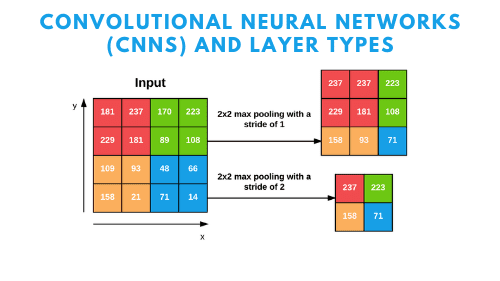
\includegraphics[width=\linewidth]{images/cnns.png}
      \caption{Convolutional neural networks} \label{fig:cnns}
    \end{subfigure}%
    \hspace*{\fill}   % maximize separation between the subfigures
    \begin{subfigure}{0.31\textwidth}
      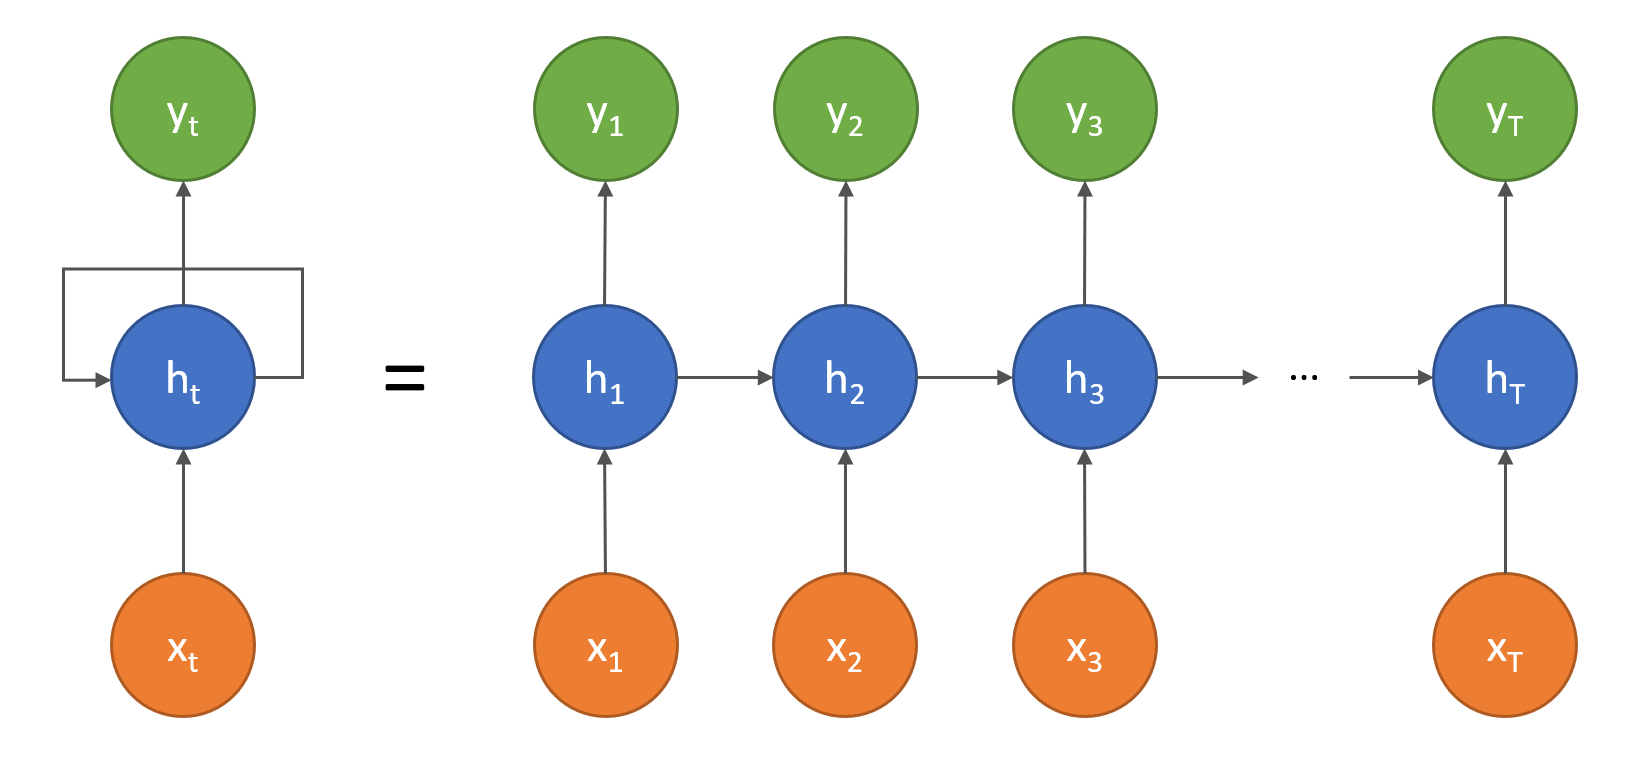
\includegraphics[width=\linewidth]{images/rnns.png}
      \caption{recurrent neural network} \label{fig:rnns}
    \end{subfigure}%
    \hspace*{\fill}   % maximizeseparation between the subfigures
    \begin{subfigure}{0.31\textwidth}
        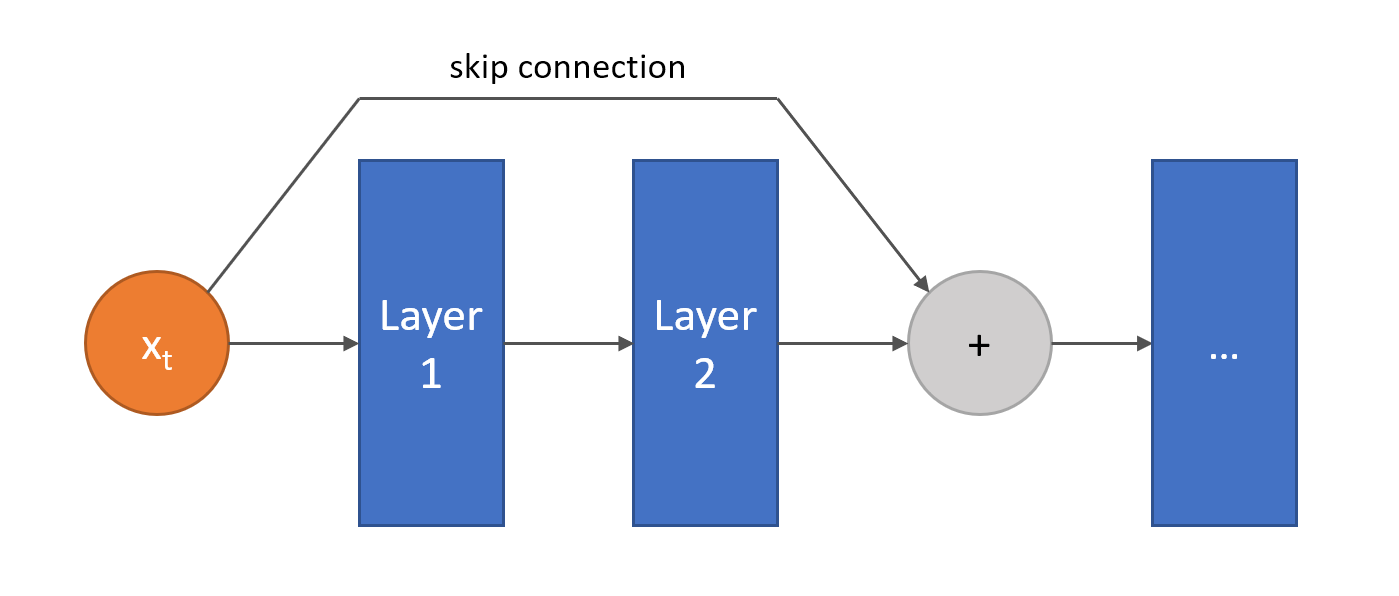
\includegraphics[width=\linewidth]{images/resnet.png}
        \caption{residual connection} \label{fig:resnet}
      \end{subfigure}%
    \hspace*{\fill}   % maximizeseparation between the subfigures
  \caption{Overview Neural Network Architectures} \label{fig:NN_architectures_Overview}
\end{figure}

Lastly, inspired by the human cognitive capabilities to focus on specific parts of an input, attention mechanisms have been introduced \cite{niu2021ReviewAttentionMechanism, aggarwal2018NeuralNetworksDeep}.
The implementation of attention in neural networks tries to address the problem of information overload, and is supposed to enable the network to allocate their resources \cite{niu2021ReviewAttentionMechanism}.
An attention mechanism has been successfully applied to various tasks in different domains, such as computer vision or natural language processing \cite{niu2021ReviewAttentionMechanism}.
The architectural realization of attention is realized differently, depending on the task at hand \cite{aggarwal2018NeuralNetworksDeep}.
The attention mechanism in computer vision involves weighting different regions of the image based on their relevance to the task \cite{aggarwal2018NeuralNetworksDeep}. 
This can be achieved through techniques such as spatial attention, channel attention or temporal attention \cite{guo2022AttentionMechanismsComputer}.
In natural language processing attention mechanism try to improve to capture the meaning of a sentence \cite{niu2021ReviewAttentionMechanism}. 
For instance, this has been achieved through the introduction of a context vector in an \gls{rnn} encoder-decoder \cite{DBLP:journals/corr/BahdanauCB14} or through self-attention \cite{vaswani2017AttentionAllYou} (see \autoref{ch:preliminaries-generativeAlgorithms-transformers} for a detailed explanation on self-attention).


\section{Deep generative Models}
\label{ch:preliminaries-generativeMlgorithms}

Deep generative \glspl{model} have revolutionized the field of artificial intelligence and machine learning by generating new and original data based on existing patterns and structures. 
Generative models try to learn a joint distribution over all the available variables \cite{kingma2019IntroductionVariationalAutoencoders}, also called the generative modeling problem \cite{goodfellow2020GenerativeAdversarialNetworks}.
Formally, in generative modeling training examples $x$ are drawn from an unkonwn distribution $p_{data}(x)$ and a generative modeling algorithm is trained to learn a distribution density function $p_{model}(x;\theta)$ that approximates the true probability density function $p_{data}(x)$ as closely as possible \cite[p. 139]{goodfellow2020GenerativeAdversarialNetworks}.
$\theta$ are the models parameters that determine the models output and usually learned by searching for $\theta$ values that result in $p_{model}$ to be as similar to $p_{data}$ as possible \cite[p. 139]{goodfellow2020GenerativeAdversarialNetworks}.

Several powerful generative modeling approaches with different architectures have emerged, each with its own strengths and weaknesses. 
This section will explore four of the most popular approaches: variational autoencoders, generative adversarial networks, transformers, and diffusion models. [TODO: label auf section]

\subsection{Variational Autoencoders}
\label{ch:preliminaries-generativeAlgorithms-variationalAutoencoders} 

In order to understand \glspl{vae} \cite{kingma2013AutoEncodingVariationalBayes}, an introduction to vanilla autoencoders is required.
Autoencoders, firstly introduced in \cite{rumelhart1986LearningInternalRepresentations}, are a neural network architecture, designed to generate a copy of the input \cite{Goodfellow-et-al-2016, Bank2020Autoencoders}.
This is done by compressing the original input $x$ into a meaningful representation by constricting the number of nodes in the intermediate hidden layer \cite{aggarwal2018NeuralNetworksDeep, Bank2020Autoencoders}, also called bottleneck.
\autoref{fig:ae} shows that an autoencoder consists of two deep-learning modules, the encoder and the decoder.
The encoder function (or generative model \cite{kingma2019IntroductionVariationalAutoencoders}), $z=f(x)$ receives an input $x$ and creates a latent representation (also called "code" \cite{aggarwal2018NeuralNetworksDeep}) with a dimensionality smaller than $x$ \cite{Goodfellow-et-al-2016, Bank2020Autoencoders}.
The decoder (or recognition model \cite{kingma2019IntroductionVariationalAutoencoders}) receives the latent representation $z$ and tries to reconstruct the original input, $r=g(z)$ with the same dimensionality as $x$ \cite{Goodfellow-et-al-2016}.
In order for the autoencoder to learn and to optimize the models parameters, a loss $L$ is calculated by applying a reconstruction loss function, that measures how close the reconstruction is to its original counterpart \cite{Bank2020Autoencoders, maheshwari2022AutoencoderIssuesChallenges}.
The reconstruction loss depends on the use case, for instance, it could be the Mean-squared error between $x$ and $r$, $L=\sum_{i=1}^{N}(x_i-r_i)^2$ for $N$ features in $x$, \cite{aggarwal2018NeuralNetworksDeep, Goodfellow-et-al-2016}.
Since $z$ is restricted in dimensionality, a simple copying from input to output, \ie $g(f(x))=x$, should not be possible and the encoder should learn to create an approximation of $x$ with its most important features \cite{aggarwal2018NeuralNetworksDeep}.
Therefore, autoencoders are a dimensionality reduction technique.
The latent representation of a fully linear autoencoder without any non-linear operations achieves the same representation as a \gls{pca} \cite{plaut2018PrincipalSubspacesPrincipal,Bank2020Autoencoders}.
Further variations of autoencoders have emerged.
Deep autoencoders expand the neural network from one hidden layer to multiple hidden layers with non-linear activation functions, further increasing the representation power \cite{aggarwal2018NeuralNetworksDeep}.
Other variants include denoising autoencoders, convolutional autoencoders or sparse autoencoders \cite{maheshwari2022AutoencoderIssuesChallenges,Goodfellow-et-al-2016}.
However, vanilla autoencoders suffer from a lack of regularity in the latent space, because they struggle with interpolation for datapoints that have not been present in the input sequence \cite{razghandi2022VariationalAutoencoderGenerativea}.

\glspl{vae} increase the reconstruction robustness by letting the decoder sample from continuos distributions \cite{kingma2013AutoEncodingVariationalBayes}.
This is achieved by introducing the \gls{kl} divergence \autoref{eqn:kl-divergence} to ensure the latent space representation follows a standard gaussian distribution (zero mean and unit variance) \cite{razghandi2022VariationalAutoencoderGenerativea, aggarwal2018NeuralNetworksDeep}.
Instead of the encoder mapping the input into a fixed vector $z$, it is mapped into a distribution, by generating two vectors representing the mean $\mu$ and standard deviation $\sigma$ of the distribution \cite{razghandi2022VariationalAutoencoderGenerativea, aggarwal2018NeuralNetworksDeep}.
Constraining the hidden representation $z$ to a gaussian distribution allows the decoder to generate new data by simply feeding samples from the standard normal distribution \cite{aggarwal2018NeuralNetworksDeep}.
However, if every object is generated from the same distribution, distinguishing between different objects or reconstructing them from a given input would be impossible.
Thus, the distribution of the encoded information $z$, conditioned on a specific input $x$, would differ from the standard normal distribution.
Hence, the constraint that the hidden representation $z$ follows a standard normal distribution would not be achieved across the encoded distribution from a single object but rather for the entire dataset \cite{aggarwal2018NeuralNetworksDeep}.
The encoder is represented as $q(z|x)$, creating the conditional distribution from which the latent vector is sampled $z\sim q(z|x)$ \cite{kingma2013AutoEncodingVariationalBayes}.
However, this stochastic sampling process makes computations non-differentiable.
In other words, the backpropagation of the gradient is not possible and our neural networks weights cannot be updated \cite{aggarwal2018NeuralNetworksDeep}.
To address this issue, a"reparameterization trick (\autoref{eqn:reparameterization}) was introduced \cite[p. 4]{kingma2013AutoEncodingVariationalBayes}.
Since $z$ is normal distributed ($z\sim N(\mu,\sigma^2)$) it can be rewritten as $z=\mu+\sigma\epsilon$ with $\epsilon$ used as an auxiliary noise variable $\epsilon \sim N(0,1)$ sampled from the standard normal distribution \cite{kingma2013AutoEncodingVariationalBayes}.

\begin{equation}
  \label{eqn:reparameterization}
  N(\mu,\sigma^2) =\mu+\sigma\epsilon
\end{equation}
\caption[Reparameterization]{Reparameterization trick}

This transformation moves the stochastic sampling process to the fixed $\epsilon$ variable and allows $\mu$ and $\sigma$ to be differentiable variables, which allows the gradient to flow and the neural network to learn \autoref{fig:vae} \cite{kingma2013AutoEncodingVariationalBayes}.
In order for the model to learn that $z$ should be close to normal distribution, a regularization loss is introduced using the \gls{kl}-divergence.
The \gls{kl}-divergence is defined as:

\begin{equation}
    \label{eqn:kl-divergence}
    KL(p\parallel q) = \sum_{i}^{N}p_i\cdot log(\frac{p_i}{q_i})
\end{equation}

with distributions $p$ and $q$.


\begin{equation}
    \label{eqn:regularization_loss}
    L_{regularization} = KL(q(z|x) \parallel p(z))
\end{equation}

The \gls{kl}-divergence is a measures how diverged two probability distributions are from one another.
Minimizing it means optimizing the parameters of $\mu$ and $\sigma$ towards resembling the distributions it is compared to.

Additionally, a reconstruction loss is computed, based on the negative log-likelihood that measuring the error between the input and output and is minimized:

\begin{equation}
    \label{eqn:reconstruction_loss}
    L_{reconstruction} =-\mathbb{E}_{q(z|x)}[logp(x|z)]
\end{equation}
with $E_{q(z|x)}$ denoting the expectation with respect to the encoder distribution.

Hence, the final loss function that is minimized during the training of the \gls{vae} is the combination both loss functions\footnote{The signs change since minimizing the negative log-likelihood is equivalent to maximizing the log likelihood. Hence, we convert the loss to a minimization loss by multiplying it with -1}:

\begin{equation}
    \label{eqn:vae_loss}
    L_{vae} =\mathbb{E}_{q(z|x)}[logp(x|z)]-KL(q(z|x) \parallel p(z))
\end{equation}



\begin{figure}
    \begin{subfigure}{0.45\textwidth}
      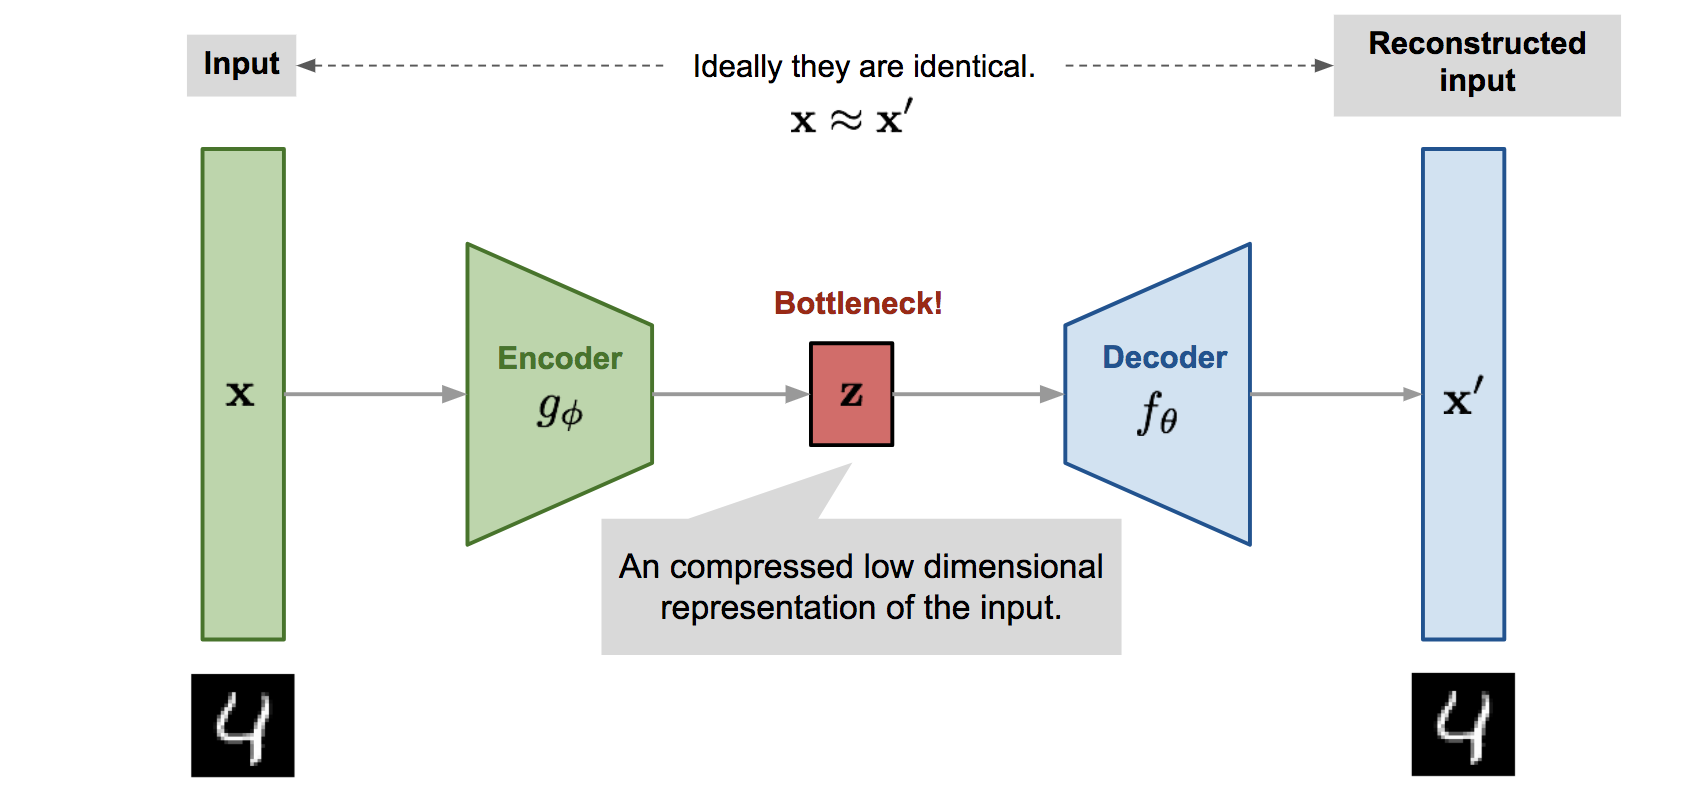
\includegraphics[width=\linewidth]{images/ae.png}
      \caption{Autoencoder} \label{fig:ae}
    \end{subfigure}%
    \hspace*{\fill}   % maximize separation between the subfigures
    \begin{subfigure}{0.45\textwidth}
      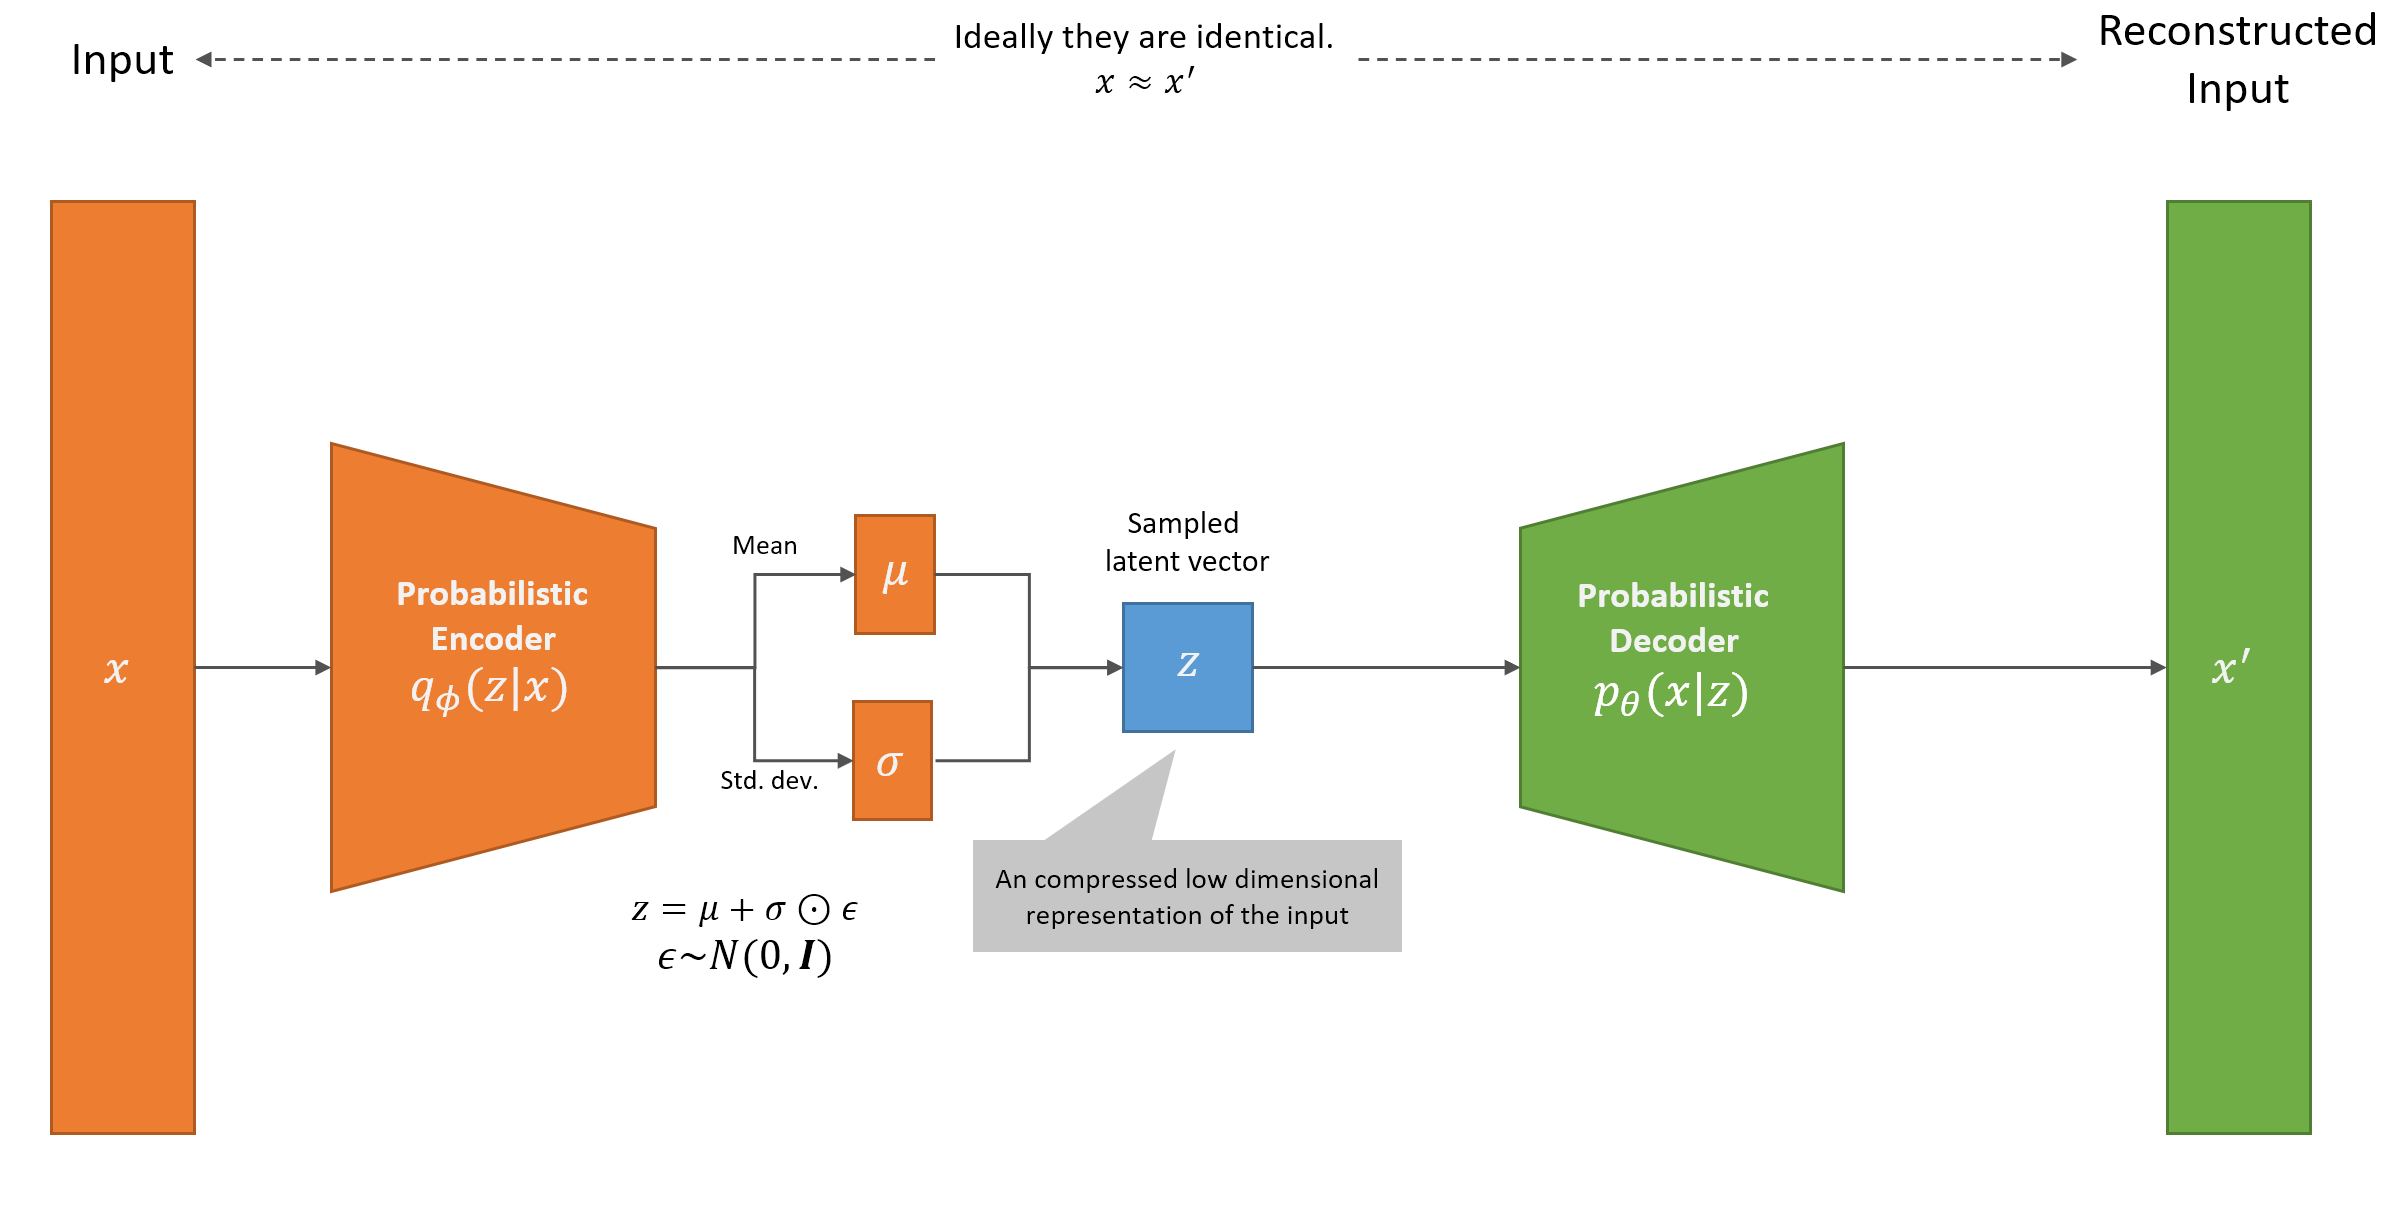
\includegraphics[width=\linewidth]{images/vae.png}
      \caption{Variational Autoencoder} \label{fig:vae}
    \end{subfigure}%
    \hspace*{\fill}   % maximizeseparation between the subfigures
  \caption{Architecture Autoencoder and Variational autoencoder} \label{fig:vae_overview}
\end{figure}
[TODO: Make sure functions in image are identical to the ones in the text]

%https://towardsdatascience.com/understanding-variational-autoencoders-vaes-f70510919f73


\subsection{Generative Adversarial Networks}
\label{ch:preliminaries-generativeAlgorithms-generativeAdversarialNetworks}

\Glspl{gan} \cite{NIPS2014_5ca3e9b1} have been introduced in 2014 as a new architecture to address the generative modeling problem.
The architecture of \Glspl{gan} is based on game theory where two \glspl{model} compete in a zero-sum min-max game \cite{NIPS2014_5ca3e9b1, zhao2022CTABGANEnhancingTabular}.
The two \glspl{model}, usually neural networks, are called the generator and the discriminator and are competing with one another.
While the generator is tasked to generate realistic looking data points, its adversary the discriminator is tasked to discriminate whether a given datapoint is a real datapoint or a fake datapoint, produced by the generator.
The generator function $G(z;\theta_G)$ with learnable parameters $\theta_G$ receives as input a vector $z$ and is tasked to transform $z$ into a realistic looking sample $x$.
An input vector $z$ is drawn from a prior distributions $p(z)$, usually a gaussian or uniform distribution, and is just an unstructured noise vector.
The fake data sample $x=G(z)$ "is intended to be statistically indistinguishable from the training data" $p_{data}$ \cite[p. 141]{goodfellow2020GenerativeAdversarialNetworks}.
The discriminator function $D(x;\theta_D)$ with learnable parameters $\theta_D$ receives as input samples $x$ that could either stem from $p_{data}$ or from $p_{model}$ generated by the generator.
Like a binary classifier, it tries to predict whether a given sample $x$ is real or fake \cite{NIPS2014_5ca3e9b1}.
The discriminators output classification is finally used in the backpropagation algorithm to update not only the discriminators parameters $\theta_D$, but also the generators parameters $\theta_G$.
So while the generator tries to produce real looking fake data samples, the discriminator tries to tell real from fake data samples apart. 
This type of training can be seen as a mentor (discriminator) providing feedback to a student (generator) on the quality of his work \cite{zhao2022CTABGANEnhancingTabular}.
Formally, the objective function $J_D$ for the discriminator that will be maximized if real $x$ are correctly classified to $1$ and fake $x$ correctly to $0$ can be defined as \cite{aggarwal2018NeuralNetworksDeep}:

\begin{equation}
    \label{eqn:discriminator}
    Maximize_DJ_D= \sum_{x\in p_{data}}^{} log [D(x)] + \sum_{x\in p_{model}}^{} log [1-D(x)]
\end{equation}

with the first part of \autoref{eqn:discriminator} handling the real data samples and the second part the synthetic data samples.
Hence, the discriminator tries to maximize correctly predicting real and fake samples as real and fake respectively.

The generator on the hand the hand tries to fool the discriminator.
Therefore, the generator tries to minimize the likelihood, that the generated fake samples are flagged as fake.
Its objective function $J_G$ is defined as \cite{aggarwal2018NeuralNetworksDeep}:
\begin{equation}
    \label{eqn:generator}
    Minimize_GJ_G= \sum_{x\in p_{model}}^{} log [1-D(x)] = \sum_{x\in p_z}^{} log [1-D(G(z))]
\end{equation}

Ultimately, the generator and the discriminator are playing a two-player minimax game with the following value function:

\begin{equation}
    \label{eqn:minmax}
    \min_G\max_DV(D,G)=\mathbb{E}_{x\sim p_{data}(x)} [log D(x)] + \mathbb{E}_{z\sim p_z(z)}[log( 1-D(G(Z)))]
\end{equation}

\autoref{eqn:minmax} is used to formulate the loss functions that are used in the training.
However, \cite{NIPS2014_5ca3e9b1} notes that in practice, \autoref{eqn:minmax} "may not provide sufficient gradient [for the generator] to learn well" \cite[p. 3]{NIPS2014_5ca3e9b1}.
This seems to be caused by the fact, that the discriminator is able to reject the early samples from the generator with a high confidence, which results in poor learning capabilities \cite{NIPS2014_5ca3e9b1}.
The proposed solution for this is to change the objective function from the generator from the minimization function \auoref{eqn:generator} to a maximization of $logD(G(z))$.
Thus, instead of minimizing the discriminator being correct, the new objective is to maximize the discriminator being wrong. 
The two loss functions $L_G$, $L_D$ that are minimized during training of the generator and discriminator respectively are defined as:

\begin{equation}
  \label{eqn:gan-loss}
  L_D=logD(x)+log(1-D(G(z)))
  L_G=-log(D(G(z)))
\end{equation}

In practice, the discriminator is trained for $k$ steps for each generator training step \cite{aggarwal2018NeuralNetworksDeep}.
This process is repeated iteratively until a nash equilibrium is reached, at which the discriminator in unable to tell real and fake samples apart ($p_{model}=p_{data}$) \cite{NIPS2014_5ca3e9b1, aggarwal2018NeuralNetworksDeep}.



\subsection{Transformers}
\label{ch:preliminaries-generativeAlgorithms-transformers}

In 2017 \cite{vaswani2017AttentionAllYou} proposed the transformer architecture for sequence modeling tasks.
While in this domain \gls{rnn} based approaches have been established state-of-the-art approaches, the newly proposed transformer architecture can be trained in a parallel manner,
overcoming the main issue of \gls{rnn}-based models, their high computational demand.
Transformers have been successfully adapted in multiple domains, such as natural language processing \cite{gillioz2020OverviewTransformerbasedModels}, computer vision \cite{khan2022TransformersVisionSurvey}, audio processing \cite{gong2022SSASTSelfSupervisedAudio} or on tabular data \cite{huang2020TabTransformerTabularData} 
and shows properties of a universal computation engine \cite{lu2021PretrainedTransformersUniversal, lin2022SurveyTransformers}.
This is achieved through the combination of several mechanism, namely, self-attention, multi-head attention, embeddings and positional encoding \cite{vaswani2017AttentionAllYou}.

The transformer model follows an encoder-decoder structure (see \autoref{fig:transformer}).
The encoder maps an input sequence to an abstract continues representation, that encapsulates all the learnt information from the input.
The decoder, in turn, utilizes this representation to generate outputs while also incorporating the previously produced output \cite{vaswani2017AttentionAllYou}.

The first step in the transformer architecture isn the transformation of the raw input through an embedding layer [TODO: verweis auf embeddings].
This Embedding allows to transform input tokens into vectors of dimension $d_{model}$ \cite{vaswani2017AttentionAllYou}.
The output of the decoder itself is used again by the decoder, for which embeddings are computed as well.
Both embeddings are combined with so-called, positional encodings.
Positional encodings have the same dimensionality as the embeddings and carry information about the positions of the tokens in the overall sequence.
\cite{vaswani2017AttentionAllYou} makes use of a $sin$ and $cos$ function to compute this vector.
The sum of the positional encoding vector and the embeddings forms the new input to the encoder or decoder.

The encoder and decoder consist of multiple blocks, named encoder-blocks and decoder-blocks respectively.
Each encoder block is based on a multi-head self-attention module, followed by a position-wise feed-forward network.
Residual connections are employed around the two sublayers, followed by a layer normalization, to facilitate building a deeper network \cite{vaswani2017AttentionAllYou, lin2022SurveyTransformers}.

A decoder block is similar to the encoder block, however, an additional multi-head attention module is added at the beginning in front of the other two-sub layers.
Additionally, the self-attention modules in the decoder are adapted in such a way, that positions are not able to attend subsequent positions (referred to as "masking" \cite[p. 3]{vaswani2017AttentionAllYou}).
This is done to ensure that predictions for a position can only depend on known outputs \cite{vaswani2017AttentionAllYou, lin2022SurveyTransformers}.

Self-attention allows the model to associate individual words in input to other words in the input.
This attention mechanism is realized using a scaled Dot-Product on query, key and value vectors ($Q$,$K$ and $V$ respectively) \cite{vaswani2017AttentionAllYou}.
All three vectors are created by sending the input through different linear layers.
The a dot product multiplication of the query and key matrixes creates a score matrix, that indicates how much focus an individual word should have on the other words, \ie how much it should attend it \cite{vaswani2017AttentionAllYou}.
The created attention matrix is finally scaled (according to key dimensionality $d_k$) and multiplied with the value vector to create the output probabilities.
The multi-head attention refers to the fact, that input is split into multiple parts before being processed by different self-attention blocks.
Outputs of the different self-attention blocks are concatenated back together afterwards \cite{vaswani2017AttentionAllYou}.
The attention mechanism can be defined as \cite[p.4]{vaswani2017AttentionAllYou}:

\begin{equation}
  \label{eqn:attention}
  Attention(Q,K,V)=softmax(\frac{QK^T}{\sqrt[]{d_k}})V
\end{equation}


\begin{figure}

  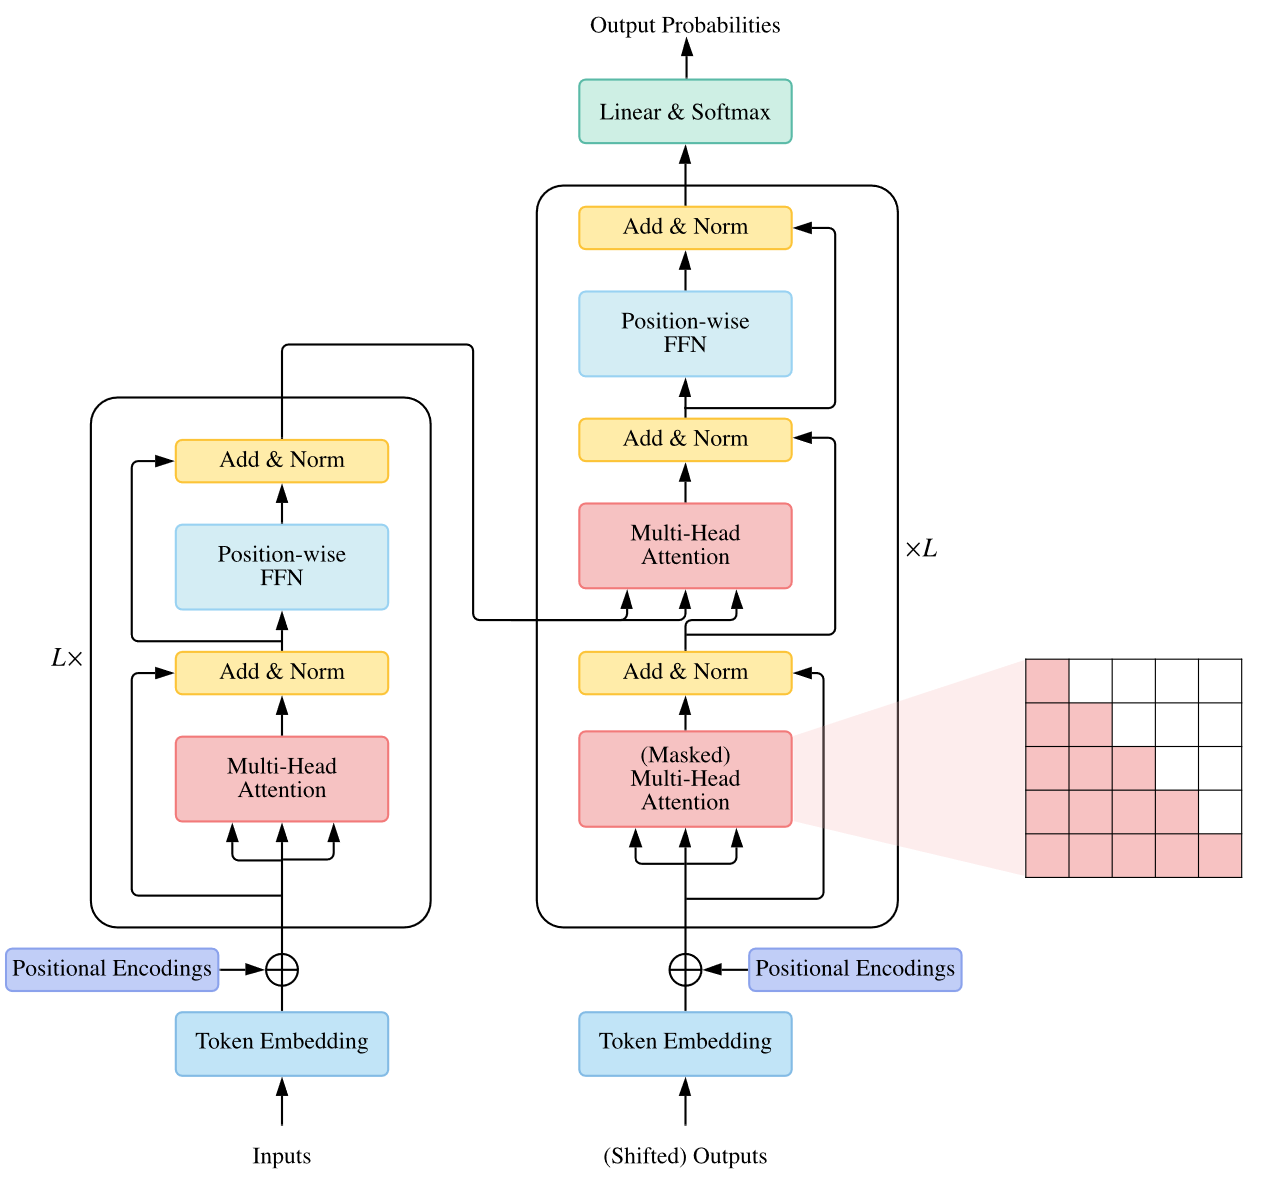
\includegraphics[width=0.8\linewidth]{images/transformer.png}

\caption{Transformer Architecture} \label{fig:transformer}
\end{figure}


\subsection{Diffusion Probabilistic Models}
\label{ch:preliminaries-generativeAlgorithms-diffusionProbabilisticModels}

\Glspl{ddpm} (from now on referred to as "diffusion models"), firstly introduced by \cite{sohl-dickstein2015DeepUnsupervisedLearning}, are a generative modeling approach inspired by non-equilibrium statistical physics \cite{sohl-dickstein2015DeepUnsupervisedLearning}.
On a high level, the whole diffusion concept can be summarized as:

\begin{quotation}
  "The essential idea, (...) is to systematically and slowly destroy structure in a data distribution through an iterative forward diffusion process. 
  We then learn a reverse diffusion process that restores structure in data, yielding a highly flexible and tractable generative model of the data." \cite[p. 1]{sohl-dickstein2015DeepUnsupervisedLearning}
\end{quotation}
Formally, \cite{ho2020DenoisingDiffusionProbabilistic} defines diffusion models as a class of \glspl{lvm} [TODO:fix] of the form $p_\theta(x_0):= \int_{}^{}p_\theta(x_{0:T})dx_{1:T}$,
with $x_1, ..., x_T$ as latents of same dimensionality as samples from the data distribution $x_0 \sim q(x_0)$.
Diffusion models consist of a forward process and a reverse process.
During the forward process, an initial data point $x0$ is obtained from the data distribution $q(x_0)$.
In the forward process (also called diffusion process), a fixed markov chain [TODO: Glossar?] gradually adds noise to the data.
$T$ defines the number of noising step and $x1,...,x_T$ denoting the latent variables, \ie the noised versions of the original data, with $x_T$ being the fully noised version of the data.
The amount of added (gaussian) noise in each timestep varies depending on the current timestep, which is controlled by a variance schedule $\beta_1, ..., \beta_T \in (0,1)$.
The forward process is defined as:


\begin{equation}
  \label{eqn:forwards_1}
  \begin{align*}
    q(x_{1:T} | x_0) := \prod_{t=1}^T q(x_t | x_{t-1}), \quad
    q(x_t | x_{t-1}) := \mathcal{N}(x_t; \sqrt{1 - \beta_t} x_{t-1}, \beta_t I)
  \end{align*}
\end{equation}

For the variance schedule it holds that if $\beta_1 < \beta_2 < ... < \beta_T$ for $t\rightarrow\infty$, the final latent $x_t$ is isotropic gaussian noise, \ie, $x_t \sim \mathcal{N}(0, \textbf{I})$, with identity matrix $\textbf{I}$.
If the reverse process is learned, this feature allows to sample from a gaussian distribution to generate new samples.
$\beta$ increases linearly in the original \gls{ddpm} approach \cite{ho2020DenoisingDiffusionProbabilistic} but was later improved to follow a cosine schedule \cite{nichol2021ImprovedDenoisingDiffusion}, improving the overall quality of the model.

\autoref{eqn:forwards_1} shows how in an iterative manner one noising step can be applied to get from $x_{t-1}$ to $x_t$ with $q(x_t | x_{t-1})$.
Through the use of a reparameterization (see \autoref{eqn:reparameterization}) and defining $\alpha := 1-\beta_t$ and $\overline{\alpha_t}:=\prod_{s=1}^{t}a_s$
Thus, the forward diffusion process can be expressed as:

\begin{equation}
  \label{eqn:forwards_2}
  \begin{align*}
    q(x_t | x_0) \quad & := \mathcal{N}(x_t; \sqrt{\bar{\alpha}_t} x_0, (1 - \bar{\alpha}_t) \textbf{I})
     &:= \sqrt{\bar{\alpha}_t} x_0 + \sqrt{1 - \bar{\alpha}_t} \epsilon \textrm{, with } \epsilon\sim\mathcal{N}(0, \textbf{I})
  \end{align*}
\end{equation}

\autoref{eqn:forwards_2} allows to compute the forward noising from $x_0$ to any timestep $t$ within one computation step, instead of iteratively applying noise over and over again.

During the reverse process, the goal is to learn the reverse distribution from noised data $x_t$ to slightly less noised data $x_{t-1}$, $q(x_{t-1}|x_t)$.
With bayes-theorem we can see that $q(x_{t-1}|x_t) = \frac{p(x_{t-1},x_t)}{p(x)}$, which means $q(x_{t-1}|x_t)$ depends on the marginal distribution of $x_t$, denoted as $p(x_t)$.
To calculate the marginal probability distribution $p(x_t)$ integration over all possible realizations of $x_{t-1}$ would be necessary, which would be computationally intractable.
As a result, $q(x_{t-1}|x_t)$ is approximated by a neural network with learnable parameters $\theta$ that learns the joint distribution $p_{\theta}(x_{0:T})$.
$p_{\theta}(x_{0:T})$ is a Marcov-chain [TODO: glossar], defined in \autoref{eqn:reverse_1}, with the transitions defined in \autoref{eqn:reverse_2}.

\begin{equation}
  \label{eqn:reverse_1}
  \begin{align*}
    p_{\theta}(x_{0:T}) := p(x_T) \prod_{t=1}^T p_{\theta}(x_{t-1} | x_t),
  \end{align*}
\end{equation}

\begin{equation}
  \label{eqn:reverse_2}
  \begin{align*}
    p_{\theta}(x_{t-1}|x_t) := \mathcal{N}(x_{t-1}; \mu_{\theta}(x_t, t), \Sigma_{\theta}(x_t, t))
  \end{align*}
\end{equation}
    
While the mean $\mu_{\theta}(x_t, t)$ is learned by the neural network, the variance $\Sigma_{\theta}(x_t, t)$ stayed fixed in the initial work by \cite{ho2020DenoisingDiffusionProbabilistic} 
but was later in \cite{nichol2021ImprovedDenoisingDiffusion} learned as well.

Like in \glspl{vae} (\autoref{ch:preliminaries-generativeAlgorithms-variationalAutoencoders}), the model is trained by minimizing its negative log-likelihood (= maximizing the log-likelihood) $-log(p_\theta(x_0))$.
$p_\theta(x_0)$ depends on all timesteps before $x_0$ and is, therefore, not tractable in practice.
As a solution, the variational lower bound on the negative log likelihood can be computed (ELBO [todo: REF]) \autoref{eqn:vlb}

\begin{equation}
  \label{eqn:vlb}
  \begin{align*}
    $-log(p_\theta(x_0)) \leq -log(p_\theta(x_0)) + KL(q(x_{1:T}|x_0) \parallel p_\theta(x_{1:T}|x_0))$
  \end{align*}
\end{equation}

The \gls{kl}-divergence (\autoref{eqn:kl-divergence}) is a non-negative measure of dissimilarity between two probability distributions. 
By minimizing the \gls{kl}-divergence as the objective function in the given inequality, the right-hand side is reduced, leading to a smaller or equal left-hand side. 
Consequently, minimizing the KL divergence  can only decrease the negative log-likelihood term on the left-hand side of the inequality. 
This implies that the objective function provides a lower bound on the log-likelihood, and any improvement in minimizing the \gls{kl}-divergence will ultimately lead to an enhancement in this lower bound.
Rewriting $KL(q(x_{1:T}|x_0) \parallel p_\theta(x_{1:T}|x_0))$ to $log(\frac{q(x_{1:T})|x_0}{p_\theta(x_{1:T}|x_0)})$ and some reformulations (see \autoref{TODO:APPENDIX}) using bayes-rule results in \autoref{eqn:vlb2}:

\begin{equation}
  \label{eqn:vlb2}
  \begin{align*}
    -log(p_\theta(x_0)) \leq log(\frac{q(x_{1:T})|x_0)}{p_\theta(x_{0:T})})
  \end{align*}
\end{equation}

\autoref{eqn:vlb2} is the variational lower bound that is minimized during training to optimizing $-log(p_\theta(x_0))$.
With additional reformulations (see \autoref{TODO:APPENDIX}), the loss function can be derived as:

\begin{equation}
  \label{eqn:vlb2}
  \begin{align*}
   $\mathbb{E}\biggl[\underbrace{D_{KL}(q(x_{T}|x_0) \parallel p(x_T))}_{L_T} + \sum_{t>1}^{} \underbrace{  D_{KL}(q(x_{t-1}|x_t,x_0) \parallel p_\theta(x_{t-1}|x_t)) }_{L_{t-1}}  \underbrace{ -log p_\theta(x_0|x_1) }_{L_{0}}\biggr]$
  \end{align*}
\end{equation}



https://www.arxiv-vanity.com/papers/2209.10948/

https://theaisummer.com/latent-variable-models/

https://matheo.uliege.be/bitstream/2268.2/15989/15/Master_thesis.pdf

https://towardsdatascience.com/understanding-diffusion-probabilistic-models-dpms-1940329d6048

https://www.youtube.com/watch?v=HoKDTa5jHvg&t=951s


% What are diffusion probabilistic models
first paper \cite{sohl-dickstein2015DeepUnsupervisedLearning}
first famouse paper \cite{ho2020DenoisingDiffusionProbabilistic}
improvements> \cite{nichol2021ImprovedDenoisingDiffusion}
follow up: \cite{dhariwal2021DiffusionModelsBeat}

\cite{ho2022ClassifierFreeDiffusionGuidance}

\cite{rombach2022HighResolutionImageSynthesis}

% mathematical formulation
% How do they work
% In what context are they used (usually image synthesis)
% Advantages / Problems / Challenges


% for tabular data
\cite{zheng2022DiffusionModelsMissing} for missing data

\cite{kotelnikov2022TabDDPMModellingTabular} tabddpm
\cite{hoogeboom2021ArgmaxFlowsMultinomial} multinomial diffusion


\subsection{Diffusion Probabilistic Models for Tabular Data}
\label{ch:preliminaries-generativeAlgorithms-diffusionProbabilisticModelsTabularData}

% How can Diffusion Probabilistic Models be used for tabular data
% Challenges of using Diffusion Probabilistic Models for tabular data (mixed data types --> different noising process, etc.)


%-------------------------------------------------------------------------
\section{Evaluation of Synthetic Tabular Data}
\label{ch:preliminaries-evaluationOfSyntheticTabularData}

- there is no universal metric for data synthesis \cite{hernandez2022SyntheticDataGeneration}
- utility and information disclosure metric dimensions \cite{goncalves2020GenerationEvaluationSynthetic}
- structural similarity \cite{elemam2020SevenWaysEvaluate}

\subsection{Statistical Evaluation}
\label{ch:preliminaries-evaluationOfSyntheticTabularData-statisticalEvaluation}

\subsection{Machine Learning Efficiency}
\label{ch:preliminaries-evaluationOfSyntheticTabularData-machineLearningEfficiency}

\subsection{Privacy Evaluation}
\label{ch:preliminaries-evaluationOfSyntheticTabularData-privacyEvaluation}

\subsection{Additional Evaluation Methods}
\label{ch:preliminaries-evaluationOfSyntheticTabularData-otherMetrics}

% Bias and stability
% Domain Expertise

\subsection{Similarity Score}
\label{ch:preliminaries-evaluationOfSyntheticTabularData-similarityScore}
% https://www.researchgate.net/publication/344227988_On_the_Generation_and_Evaluation_of_Tabular_Data_using_GANs

% TOREAD: https://www.researchgate.net/publication/361949372_TabSynDex_A_Universal_Metric_for_Robust_Evaluation_of_Synthetic_Tabular_Data

%-------------------------------------------------------------------------




